%  article.tex (Version 3.3, released 19 January 2008)
%  Article to demonstrate format for SPIE Proceedings
%  Special instructions are included in this file after the
%  symbol %>>>>
%  Numerous commands are commented out, but included to show how
%  to effect various options, e.g., to print page numbers, etc.
%  This LaTeX source file is composed for LaTeX2e.

%  The following commands have been added in the SPIE class 
%  file (spie.cls) and will not be understood in other classes:
%  \supit{}, \authorinfo{}, \skiplinehalf, \keywords{}
%  The bibliography style file is called spiebib.bst, 
%  which replaces the standard style unstr.bst.  

\documentclass[]{spie}  %>>> use for US letter paper
%%\documentclass[a4paper]{spie}  %>>> use this instead for A4 paper
%%\documentclass[nocompress]{spie}  %>>> to avoid compression of citations
%% \addtolength{\voffset}{9mm}   %>>> moves text field down
%% \renewcommand{\baselinestretch}{1.65}   %>>> 1.65 for double spacing, 1.25 for 1.5 spacing 
%  The following command loads a graphics package to include images 
%  in the document. It may be necessary to specify a DVI driver option,
%  e.g., [dvips], but that may be inappropriate for some LaTeX 
%  installations. 
\usepackage[]{graphicx}

\usepackage{subfig}
\usepackage{verbatim}
\usepackage{amsmath}
\usepackage{amssymb}
\usepackage{algpseudocode}
\usepackage{algorithm}

\newcommand{\stdfigure}[3]{ \begin{figure}[htp] \centering \includegraphics[width=0.95\linewidth]{#1} \caption{#3} \label{fig:#2} \end{figure} }
\newcommand{\stdfigurevar}[4]{ \begin{figure}[htp] \centering \includegraphics[width=#4\linewidth]{#1} \caption{#3} \label{fig:#2} \end{figure} }
\newcommand{\stdfigurefull}[3]{ \begin{figure*}[htp] \centering \includegraphics[width=0.95\linewidth]{#1} \caption{#3} \label{fig:#2} \end{figure*} }
\newcommand{\stdfigurefullvar}[4]{ \begin{figure*}[htp] \centering \includegraphics[width=#4\linewidth]{#1} \caption{#3} \label{fig:#2} \end{figure*} }

\newcommand{\fig}[1]{Figure~\ref{fig:#1}}
\newcommand{\figf}[1]{Figure~\ref{fig:#1}}
\newcommand{\figsub}[2]{Figure~\ref{fig:#1}\,(#2)}
\newcommand{\figsubf}[2]{Figure~\ref{fig:#1}\,(#2)}
\newcommand{\figsubref}[2]{Figure~\ref{fig:#1}\,\subref{fig:#2}}
\newcommand{\figsubreff}[2]{Figure~\ref{fig:#1}\,\subref{fig:#2}}
% not figure how to remove () from subref
\newcommand{\figsubrefrange}[3]{Figure~\ref{fig:#1}\,\subref{fig:#2}-\subref{fig:#3}}
\newcommand{\figsubrefrangef}[3]{Figure~\ref{fig:#1}\,\subref{fig:#2}-\subref{fig:#3}}

\newcommand{\eq}[1]{Eq.~(\ref{eq:#1})}
\newcommand{\eqf}[1]{Equation~(\ref{eq:#1})}

\newcommand{\sect}[1]{Section~\ref{sec:#1}}
\newcommand{\sectf}[1]{Section~\ref{sec:#1}}

\newcommand{\tbl}[1]{Table~\ref{tbl:#1}}
\newcommand{\tblf}[1]{Table~\ref{tbl:#1}}

\newcommand{\dataset}[1]{Dataset~#1}
\newcommand{\datasetf}[1]{Dataset~#1}

\newcommand{\alg}[1]{Algorithm~\ref{alg:#1}}
\newcommand{\algf}[1]{Algorithm~\ref{alg:#1}}
% \newcommand{\algl}[2]{Algorithm~\ref{alg:#1} line #2}
% \newcommand{\alglf}[2]{Algorithm~\ref{alg:#1} line #2}
% \newcommand{\algls}[2]{Algorithm~\ref{alg:#1} lines #2}
% \newcommand{\alglsf}[2]{Algorithm~\ref{alg:#1} lines #2}
\newcommand{\lne}[1]{line~\ref{ln:#1}}
% \newcommand{\lns}[1]{lines #1}
% \newcommand{\lnf}[1]{Line #1}
% \newcommand{\lnsf}[1]{Lines #1}

\newcommand{\red}[1]{\textcolor{red}{#1}}
\newcommand{\yellow}[1]{\textcolor{red}{#1}}
\newcommand{\green}[1]{\textcolor{green}{#1}}

\newcommand{\rem}[1]{\pdfmarkupcomment[markup=StrikeOut,color=red,author=JW]{#1}{removed}}
% \newcommand{\add}[1]{\pdfmarkupcomment[markup=Highlight,author=JW,color=yellow,opacity=1.0]{#1}{added}}
\newcommand{\add}[1]{\yellow{#1}}
% \newcommand{\upd}[1]{\pdfmarkupcomment[markup=Highlight,author=JW,color=green,opacity=1.0]{#1}{to update}}
\newcommand{\upd}[1]{\green{#1}}
\newcommand{\com}[2]{\pdfmarkupcomment[markup=Highlight,author=JW,color=blue,opacity=1.0]{#1}{#2}}

\newcommand{\ncite}[1]{}
\newcommand{\ncaption}[1]{}

\newcommand{\prop}[1]{Property~(#1)}
\def\props{properties}
\def\fprops{Properties}

\def\data{unary}
\def\smooth{binary}
\def\dataf{Unary}
\def\smoothf{Binary}

\def\obj{substructure}

\def\pslice{U_k}
\def\nslice{U_{k+1}}

\def\eg{e.g.}
\def\etal{et al.}
\def\etc{etc.}
\def\ie{i.e.}

\title{Interactive Grain Image Segmentation using Graph Cut Algorithms} 

%>>>> The author is responsible for formatting the 
%  author list and their institutions.  Use  \skiplinehalf 
%  to separate author list from addresses and between each address.
%  The correspondence between each author and his/her address
%  can be indicated with a superscript in italics, 
%  which is easily obtained with \supit{}.

\author{Jarrell Waggoner\supit{a}, Youjie Zhou\supit{a}, Jeff Simmons\supit{b}, Ayman Salem\supit{b}, \\ Marc De Graef\supit{c}, and Song Wang\supit{a}
\skiplinehalf
\supit{a}University of South Carolina, Columbia, SC 29208, USA; \\
\supit{b}Materials and Manufacturing Directorate, Air Force Research
Labs, Dayton, OH 45433, USA; \\
\supit{c} Carnegie Mellon University, Department of Materials Science and Engineering, 5000 Forbes Avenue, Pittsburgh, PA, 15213, USA
}

%>>>> Further information about the authors, other than their 
%  institution and addresses, should be included as a footnote, 
%  which is facilitated by the \authorinfo{} command.

\authorinfo{Further author information: (Send correspondence to J.W.)\\
J.W.: E-mail: waggonej@email.sc.edu, Telephone: 847-261-4747\\ 
Y.Z.: E-mail: zhou42@email.sc.edu \\ 
J.S.: E-mail: jeff.simmons@wpafb.af.mil \\ 
A.S.: E-mail: ayman.salem.ctr@wpafb.af.mil \\ 
M.G.: E-mail: degraef@cmu.edu \\
S.W.: E-mail: songwang@cec.sc.edu, Telephone: 803-777-2487}
%%>>>> when using amstex, you need to use @@ instead of @


%%%%%%%%%%%%%%%%%%%%%%%%%%%%%%%%%%%%%%%%%%%%%%%%%%%%%%%%%%%%% 
%>>>> uncomment following for page numbers
% \pagestyle{plain}    
%>>>> uncomment following to start page numbering at 301 
%\setcounter{page}{301} 
 
  \begin{document} 
  \maketitle 

%%%%%%%%%%%%%%%%%%%%%%%%%%%%%%%%%%%%%%%%%%%%%%%%%%%%%%%%%%%%% 
\begin{abstract}
% \input{spie-abstract.tex}
Segmenting materials images is a laborious and time-consuming process
and automatic image segmentation algorithms usually contain
imperfections and errors.  Interactive segmentation is a growing topic
in the areas of image processing and computer vision, which seeks to
find a balance between fully automatic methods and fully-manual
segmentation processes. By allowing minimal and simplistic interaction
from the user in an otherwise automatic algorithm, interactive
segmentation is able to simultaneously reduce the time taken to
segment an image while achieving better segmentation results. Given
the specialized structure of materials images and level of
segmentation quality required, we show an interactive segmentation
framework for materials images that has two key contributions: 1) a
multi-labeling framework that can handle a large number of structures
while still quickly and conveniently allowing manual interaction in
real-time, and 2) a parameter estimation approach that prevents the
user from having to manually specify parameters, increasing the
simplicity of the interaction.  We show a full formulation of each of
these contributions and example results from their application.
\end{abstract}

%>>>> Include a list of keywords after the abstract 

\keywords{Segmentation, Materials, Propagation, Interactive, Graph-Cut}

%%%%%%%%%%%%%%%%%%%%%%%%%%%%%%%%%%%%%%%%%%%%%%%%%%%%%%%%%%%%%

\section{Introduction}
\label{sec:intro}

Interactive segmentation is a rapidly-growing area of Computer Vision
and has seen heightened interest recently\cite{kuang:12,straehle:12}.
While traditional segmentation seeks to identify objects/structures
within an image in a fully-automated fashion, interactive
segmentation, similar to Active Learning~\cite{settles:09},
accomplishes the same goal using a sparse number of user interactions
which are incorporated directly into the algorithm, including the
approaches/models used to perform the segmentation.  These
interactions may take on different forms, and may include drawing a
bounding box~\cite{rother:04}, roughly outlining a
boundary~\cite{mortensen:95}, or drawing brush strokes inside and/or
outside the object of interest~\cite{santner:10, unger:08, boykov:01b,
  vezhnevets:95}.  A desired property of an interactive segmentation
approach is that the user interaction be as convenient (\ie low
cognitive load) and sparse (\ie few in number) as possible, while
simultaneously providing immediate feedback to the user on every
interaction.

Many existing methods segment the object of interest using a model
learned from user interactions~\cite{boykov:01b, unger:08, rother:04}.
Other approaches incorporate interaction into morphological operations
(watershed)~\cite{straehle:12}, co-segmentation~\cite{batra:10}, or
incorporate machine-learning to aid in the interactive
process~\cite{top:11, kuang:12}.  These interactive methods have been
applied to a number of domains, including natural
images~\cite{rother:04}, medical images~\cite{boykov:00}, and
neuroimages~\cite{straehle:11, straehle:12}.

One domain that has been unaddressed in interactive segmentation
literature is Materials Science image segmentation, where there are no
existing techniques focusing solely on segmenting materials images
using an interactive approach.  Materials science is especially
important to the development of new metals and biomaterials, and
presents unique challenges in image segmentation.  First, materials
images are often segmented in volumes~\cite{ibrahim:91} consisting of
individual image ``slices'' along the z-axis, as shown by the two
sample slices in \fig{full-ex}, producing numerous images that must
all be segmented to fully and properly analyze the volume.  Second,
depending on the inter-slice distance, a slice may share large overlap
with its neighboring slices.  This results in slices being very
coherent from one slice to the next, requiring that segmentation
methods handle this coherency to obtain accurate segmentation.  Third,
materials volumes consist of numerous substructures (\eg,``grains'' in
a metallic material, or ``cells'' in a biomaterial, etc.) with complex
relationships (\eg, adjacency/nonadjacency relationships) among them
that determine many desirable properties of the
material~\cite{swiler:95, rollett:04}.  Existing interactive
segmentation techniques often focus on only foreground-background
segmentation~\cite{rother:04, boykov:01b}, and may not scale to the
large number of substructures present in materials images.  Other
methods may handle multiple structures~\cite{straehle:11,
  straehle:12}, but do not incorporate any prior knowledge about the
unique relationships among substructures~\cite{reed:06, tan:04}.
Finally, the imaging techniques used to obtain a materials image
volume may result in significant noise or other ambiguities that makes
fully-automated segmentation difficult or impossible.  As we discuss
next, existing techniques do not address all of these challenges.

There are a number of existing, non-interactive approaches to segment
materials images~\cite{chuang:08, simmons:09}.  Among the most
prominent is the work of Comer~\etal~\cite{comer:94, comer:00} on the
EM/MPM algorithm, originating from~\cite{marroquin:87} .  Other
methods that have been specifically used on materials images include
graph cut~\cite{landis:11, waggoner:11}, stabilized inverse diffusion
equations~\cite{huffman:08}, Bayesian methods~\cite{comer:11,
  simmons:08}, and the watershed~\cite{liq:07} method.  Most often,
materials images are opportunistically segmented by the simplest tools
available, such as thresholding~\cite{gonzalez:08,shapiro:01}, or
out-of-the-box methods such as watershed or normalized cut.  All of
these techniques are able to achieve reasonable results in a
fully-automated fashion, however, they do not incorporate any
interaction for manual refinement by a user.  Since some of these
approaches may require significant time to run, requiring the user to
examine and correct problems only after the algorithm is complete may
not be practical if rapid refinement is desired.  Conversely, the
interactive segmentation techniques discussed previously do not
incorporate any specific domain knowledge about materials images, and
thus may require additional effort on the part of the user than may
otherwise be needed when segmenting a materials image volume.

In this paper, we present an interactive segmentation approach to
segment materials science image volumes.  We show that an existing
propagation-based materials image segmentation
approach~\cite{waggoner:11} can be extended to allow for convenient
interactive segmentation.  We illustrate the performance of the
proposed approach by using it to segment a materials image volume
using smaller number of interactions compared with general interactive
segmentation methods that do not incorporate materials-specific
priors.  Finally, we develop methods to estimate the parameters of
this proposed approach to further reduce the number of user-required
interactions in the segmentation process.

The remainder of this paper is organized as follows: in
\sect{interactive} we discuss the proposed interactive segmentation
approach for materials image volumes. In \sect{param}, we show how
some of the parameters of the proposed method.  In \sect{ex}, we
evaluate the proposed method's performance against another interactive
segmentation method.  Finally, in \sect{conclusion} we provide brief
concluding remarks.

\section{Interactive Materials Segmentation}
\label{sec:interactive}

In~\cite{waggoner:11} we develop a volume segmentation method which
was formulated as a propagation from the segmentation initialization
$S^U$ of a slice $U$ through the remaining slices to segment the
complete volume.  This propagation was done while preserving the
topology (\ie, non-adjacency relations among segments), which led to a
better performance when compared with methods that did not incorporate
topology as a prior.  More formally, we define propagation as the
processing of transferring a known segmentation to the remaining
unsegmented slices.
\begin{figure}[htbp]
\centering
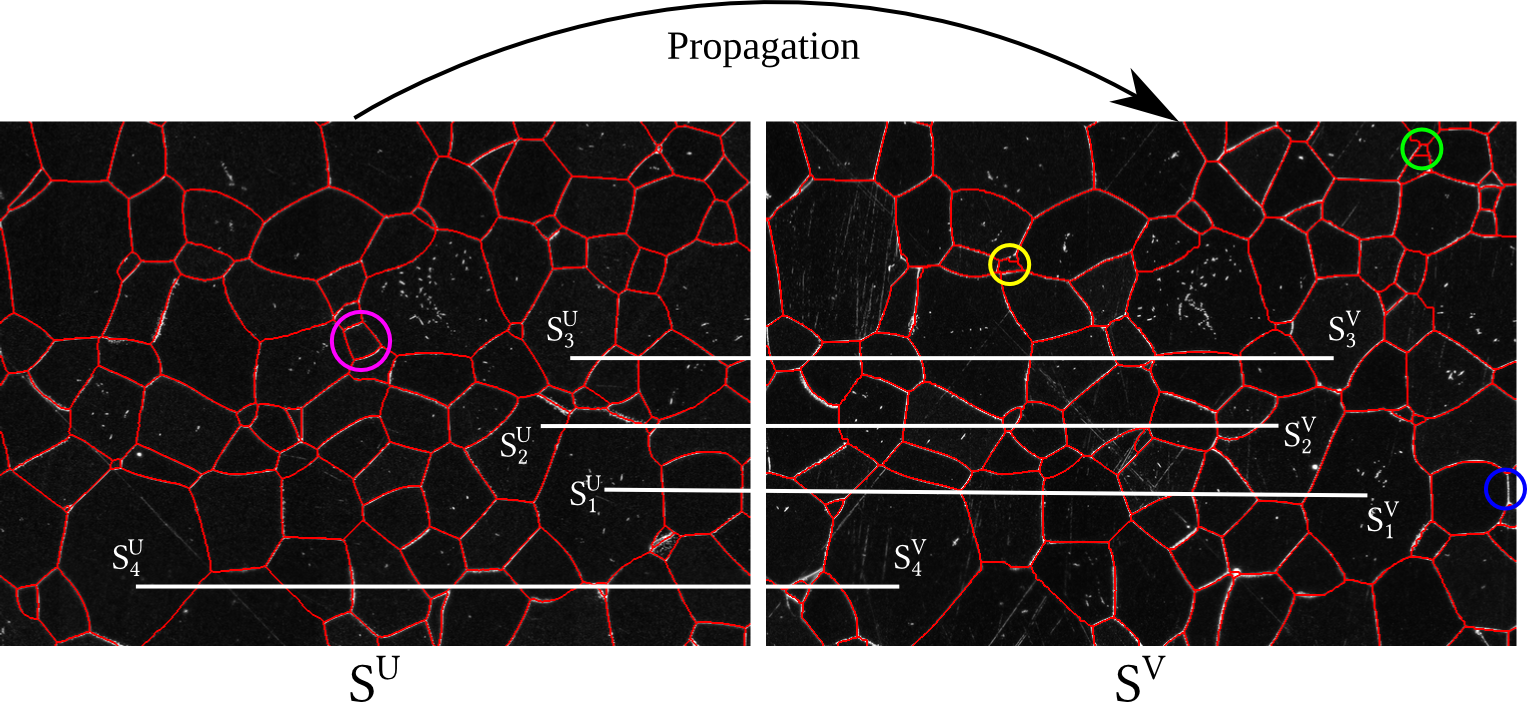
\includegraphics[width=\linewidth]{fig/dd}
\caption{Example of segmentation propagation, highlighting different
  types of topology changes.  Further discussion in the
  text.} \label{fig:full-ex}
\end{figure}
Specifically this known segmentation $S^U$ is made up of segments
$S^U_i$,
\[S^U = \{ S^U_1, S^U_2, \ldots, S^U_n \} \]
where this collection of segments makes up a partition of the slice
$U$,
\[ U = \bigcup_{i=1}^{n} S^U_i . \] This is shown by the many
``grain'' structures in \fig{full-ex} separated by red lines.
Segmentation $S^U$ is transferred to an unknown image $V$ to yield
segmentation $S^V$.  In our previous method, this was done using an
energy minimization formulation of the form
\begin{equation}
  E( S^V ) = \sum_{p\in V}\Theta_p(S^V_i) + 
  \sum_{\{p,q\}\in\mathcal{P}^V_n} \Phi_{pq}(S_i^V , S_j^V) .
\label{eq:energy1}
\end{equation}
where $\mathcal{P}^V_n$ the set of all 4-connected pixels.  The the
\data{} term $\Theta_p(S^V_i)$, which represents a cost for a pixel
$p$ being assigned to a segment $S^V_i$, was set using a dilation from
the initialization $S^U$, \ie, all pixels within a constant distance
$d$:
\begin{equation}
  \Theta_p(S^{V}_i) = \left\{
    \begin{array}{lcr}
      0, &  \textrm{distance}(p,S^U_i) < d  \\
      \infty, & \textrm{ otherwise} \\
    \end{array}
  \right.
  \label{eq:theta}
\end{equation}
In addition, the \smooth{} term $\Phi_{pq}(S_i^V , S_j^V)$, which
represents a cost for a pair of pixels $p,q$ being assigned two
(possibly the same) segments $S^V_i, S^V_j$, was constrained to
preserve \emph{non-adjacency} among the different segments; \ie, any
two segments $S^V_i, S^V_k$ are allowed to be adjacent (have pixels
that are 4-connected between them) if the corresponding segments in
$S^U_i, S^U_k$ were also adjacent,
\begin{equation} \Phi_{pq}(S^V_i , S^V_j) = \left\{
    \begin{array}{lcr}
      0, & i = j \\
      \infty, & \{ S^U_i, S^U_j \} \notin \mathcal{A}^U  \\
      g( p, q ), & \{ S^U_i, S^U_j \} \in \mathcal{A}^U \\
    \end{array}
  \right. ,
  \label{eq:phi}
\end{equation}
where $\mathcal{A}^U$ contains segment pairs that are adjacent in
$S^U$.  An example is shown in \fig{full-ex}, where $S^V_1$ and $S^V_2$
are allowed to be adjacent because $S^U_1$ and $S^U_2$ were adjacent
in $S^U$.  However, $S^V_1$ and $S^V_4$ have an infinity penalty
because $S^U_1$ and $S^U_4$ are not adjacent in $S^U$.  This topology
constraint was found to be particularly important for materials
images, and our proposed method was able to outperform other methods
that did not incorporate such a prior.

This formulation was shown to be minimizable to a local
optimum~\cite{veksler:99, boykov:01}.  However, one phenomenon that
was observed in this previous work was that, during propagation,
topology might not be fully consistent.  For example, a new structure
that was not present in the known slice $S^U$ might appear in $S^V$,
\eg the structure in the yellow circle in \fig{full-ex}.  Similarly,
a structure in $S^U$ might not be present in $S^V$, such as the
structure circled in magenta in \fig{full-ex}.  This breaks the
topology constraints given in \eq{phi}, which leads to segmentations
where spurious segments are left behind, as shown by the structure
circled in green in \fig{full-ex}, or newly-appearing structures are
not given an independent segment, as shown by the structure circled in
blue in \fig{full-ex}.  The previous method made use of a brute-force
automated approach to identify structures that were ``appearing'' or
``disappearing'' in the new slice $S^V$, and add or remove them,
respectfully.  However, particularly when the inter-slice distance is
too large, it is not possible to predict every location where such
structures may appear or disappear.  Thus, for the proposed
interactive segmentation we discuss in this paper, our desire is to
\emph{resegment} the segmentation $S^V$ by interactively allowing the
user to specify areas for correction (\ie structures that should have
disappeared, or were not identified in $S^V$) and producing a
corrected $S^{\tilde{V}}$ segmentation for the same image $V$.  We
propose to allow the user to correct these two types of segmentation
errors within this framework by: 1) annotating the location of a new
segment to handle cases where a new structure appears in slice $V$,
and 2) annotation of existing segments that should no longer be
present in segmentation $S^V$.  % These cases correspond to the
% aforementioned cases where a substructure did not dissappear as it
% should, or a new appearing structure was not identified, respectively.
Other errors, such as misplaced boundaries, can be corrected by
combinations of the above operations, \eg, merging two segments and
then introducing a new segment at the correct location.

These interactions are inherently local, since the human annotation
only affects a small area within the larger image.  The previous
propagation method segmented entire slices, which was more
computationally intensive than is desirable in an interactive system,
which should respond instantaneously to user feedback.  So, to make
our interactive system more responsive when the user is providing
annotations, we wish to restrict our interactive operations to small,
local regions within a segmentation instead of resegmenting the entire
image with the new annotations.  We will further discuss the two
approaches, and how we identify local regions for each, in the
following subsections.

\subsection{Removal}
\label{sec:remove}

We allow the user to select a specific segment $S^V_k$ for removal by
interactively clicking on this segment in a visualized segmentation.
Instead of naively removing this segment by arbitrarily merging it
into one of its neighbors, we use the same energy minimization
discussed above to assign segments to each individual pixel.  We do
this by finding a local group of segments around the removed segment
(selected by the user), as shown by $S^V_1, S^V_2, S^V_3$ surrounding
the removed segment $S^V_k$ in \figsub{removal-ex}{a}, and re-run the
energy minimization within this local region after modifying the
$\Theta$ term to incorporate the interaction, resulting in
\figsub{removal-ex}{b}.
\begin{figure}[htbp]
\centering
\subfloat[]{
\includegraphics[width=0.33\linewidth]{fig/aaa.pdf}}
\hspace{0.1em}
\subfloat[]{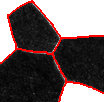
\includegraphics[width=0.33\linewidth]{fig/aac}}
\caption{Example selection of $S^V_k$ for removal.  \textbf{(a)}
  Chosen $S^V_k$ and surrounding segments.  \textbf{(b)} Local region
  extracted and energy minimized in this
  region.} \label{fig:removal-ex}
\end{figure}

To identify the local neighborhood in which we should run the proposed
interactive segmentation for segment removal, we must first identify
the neighbors of the removed segment.  For ease of notation, we use
similar notation to the adjacency definition above by using
$\{\mathcal{A}^V\}_k$ to refer to the set of segments neighboring a
particular segment $S^V_k$.  So by grouping all the pixels in the
removed segment and its adjacent segments, we form the local region on
which we run the energy minimization,
\begin{equation}
  \mathcal{L} = \{\mathcal{A}^V\}_k \bigcup S^V_k .
\end{equation}

To update the $\Theta$ term in the energy minimization, we incorporate
these adjacent neighbors by allowing all the pixels in the removed
segment $p\in S^V_k$ to be assigned any of its neighboring label's
segments, \ie,
\begin{equation}\label{eq:remove}
\begin{aligned}
 \forall p \in S^V_k ,& \quad \Theta_p(S^{\tilde{V}}_i) = \left\{
   \begin{array}{lcr}
     0, & S^V_i \in \mathcal{A}_k \textrm{ and } i \neq k  \\
     \infty, & \textrm{ otherwise} \\
   \end{array}
 \right. \\
\forall p \notin S^V_k ,& \quad \Theta_p(S^{\tilde{V}}_i) = \Theta_p(S^V_i)
\end{aligned}
\end{equation}
% \begin{align*}
%  \forall p \in S^V_k , & \\
%  % & \Theta_p(S^{\tilde{V}}_k) = \infty \\
%  & \Theta_p(S^{\tilde{V}}_i) = \left\{
%    \begin{array}{lcr}
%      0, & S^V_i \in \mathcal{A}_k \textrm{ and } i \neq k  \\
%      \infty, & \textrm{ otherwise} \\
%    \end{array}
% \right. % , \textrm{ where } i \neq k
% \\
% \forall p \notin S^V_k , & \\ 
% & \Theta_p(S^{\tilde{V}}_i) = \Theta_p(S^V_i)
% \end{align*}
which results in all pixels $p$ that were previously in $S^V_k$ being
assigned an $\infty$ penalty in $S^{\tilde{V}}$, while being given a
$0$ cost if they are assigned to the neighbors of $S^V_k$ in
$S^{\tilde{V}}$.  For other pixels $p\notin S^V_k$, their costs in
$S^{\tilde{V}}_k$ remain exactly as they were in $S^V_k$.  By updating
$\Theta$ in this fashion, we reassign the segments surrounding $S^V_k$
to all of its pixels, but we do not require that $S^V_k$ be reassigned
to a single segment.  Thus the energy minimization may reassign the
some pixels in $S^V_k$ to one segment, and other pixels to another
segment, as shown in \figsub{removal-ex}{b}.

The interaction required by the user for removal of a segment is very
minimal---a single click anywhere inside of the desired $S^V_k$
segment is all that is necessary for the system to complete the
operation.  The full algorithm for removal is shown in \alg{remove}.

\begin{algorithm}[!t]
  \centering
  \algrenewcommand\algorithmicforall{\textbf{for each}}
  \begin{algorithmic}[1]
    \Function{RemoveSegment}{$S^V, S^V_k$}
    % \State $A_k \gets$ neighbors for $S^V_k$
    \State $\mathcal{L} \gets \{\mathcal{A}^V\}_k \bigcup S^V_k$
    \State $\forall p \in \mathcal{L}$, build graph for energy minimization problem from~\cite{waggoner:11}
    \State $\Theta \gets $ set from \eq{remove}
    \State $S^{\tilde{V}} \gets S^V$ updated with the pixels assigned in $\mathcal{L}$
    \State \textbf{return} updated $S^{\tilde{V}}$
    \EndFunction
  \end{algorithmic}
  \caption{Interactively specifying segment to remove.}
  \label{alg:remove}
\end{algorithm}

\subsection{Addition}
\label{sec:addition}

Unlike removal, interactively annotating an additional structure
cannot be solely formulated as a simple modification of the $\Theta$
term in the energy minimization formulation.  This is because the
multi-labeling problem used to optimize the energy minimization form
in~\cite{waggoner:11} optimizes over a fixed set of segments, and
cannot create new segments.  Thus, we must explicitly create a new
segment at the location specified by the user.

We take as input from the user, an annotation specifying the center
location $c$ of the new segment $S^{\tilde{V}}_{n+1}$.  In addition to
this, we also accept two parameters from the user: 1) the \emph{seed}
distance $s$ specifying a circular region within the interior to the
desired structure to be segmented; 2) a \textit{dilation} parameter
$d$, which is the same as the dilation parameter used
in~\cite{waggoner:11}, which should completely cover the structure to
be segmented.  We explicitly enforce that $d \geq s$ for any choice of
$s$.

We call pixels within the seed distance $s$ of the added point ``seed
pixels'' and pixels within the dilation distance $d$ of the added
point ``dilation pixels.''  Using this approach, seed pixels are
\emph{guaranteed} to be part of the added segment, as shown by the
green circle in \figsub{addition-ex}{b}, and dilation pixels are
\emph{potentially} part of the added segment, as shown by the blue
circle in \figsub{addition-ex}{b}.  This makes these parameter
conceptually simple for the user to tune.  In \sect{param}, we discuss
how to automate the selection of these parameters to further reduce
the user's burden when interactively segmenting a materials volume.

\begin{figure}[htbp]
\centering
\subfloat[]{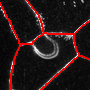
\includegraphics[width=0.30\linewidth]{fig/bba}}
\hspace{0.1em}
\subfloat[]{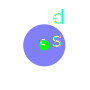
\includegraphics[width=0.30\linewidth]{fig/bbb.pdf}}
\hspace{0.1em}
\subfloat[]{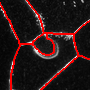
\includegraphics[width=0.30\linewidth]{fig/bbc}}
\caption{Annotating the addition of a segment.  \textbf{(a)}
  Segmentation $S^V$ with a structure that has no corresponding
  segment.  \textbf{(b)} Annotation of a center point $c$, along with
  a seed distance $s$ and a dilation distance $d$.  \textbf{(c)} The
  result of running the proposed method using the annotation from
  (b).} \label{fig:addition-ex}
\end{figure}

Since we define segmentation $S^V$ as having $n$ segments $S^V_1,
S^V_2, \ldots, S^V_n$, we introduce a new $S^V_{n+1}$ segment in the
updated segmentation $S^{\tilde{V}}$.  This segment
$S^{\tilde{V}}_{n+1}$ is introduced by giving a zero cost for all
pixels within the dilation distance of the added point $c$, \ie
\begin{equation}
  \label{eq:d}
  \Theta_p(S^{\tilde{V}}_{n+1}) = \left\{
    \begin{array}{lcr}
      0, & \| p - c \| \leq d  \\
      \infty, & \textrm{ otherwise} \\
    \end{array}
  \right.
\end{equation}
where $\| \cdot \|$ is the euclidean distance between $p$ and $c$.
Though this is necessary to include the new segment in the energy
minimization, it is not sufficient to guarantee that it will appear in
the final segmentation.  To insure that some of pixels near the added
point are guaranteed to be part of the segmentation, we give an
infinity penalty for pixels within the seed distance $s$ to be
assigned any other segment except $S^{\tilde{V}}_{n+1}$.  Similar to
\eq{d} above, we set
\begin{equation}
  \label{eq:s}
  \Theta_p(S^{\tilde{V}}_i) = \left\{
    \begin{array}{lcr}
      \infty, & \| p - c \| \leq s \textrm{ and } i \neq n+1  \\
      \Theta_p(S^{V}_i), & \textrm{ otherwise} \\
    \end{array}
  \right.
\end{equation}
which \emph{fixes} pixels within the seed distance $s$ of the added
point to be assigned only to $S^{\tilde{V}}_{n+1}$; if they are not,
then they take on the same value as they did in the energy
minimization in $S^V$.  Similar to the removal step in \sect{remove},
we can also do this procedure in a local region for efficiency by
finding all segments within the seed distance $s$ of $c$ and find all
adjacent segments to these segments to form the local region.  For
ease of notation, we use $\{\mathcal{A}^V\}_{c|s}$ to refer to the set
of all segments within a distance $s$ to point $c$.  The full
algorithm for introducing additional segments is shown in
\alg{addition}.
\begin{algorithm}[!t]
  \centering
  \algrenewcommand\algorithmicforall{\textbf{for each}}
  \begin{algorithmic}[1]
    \Function{AddSegment}{$S^V, c_{x,y}$, $s$, $d$}
    \State $\mathcal{L} \gets \{\mathcal{A}^V\}_{c|s}$
    \State $\forall p \in \mathcal{L}$, build graph for energy minimization problem from~\cite{waggoner:11}
    \State $\Theta \gets $ set from \eq{d} and \eq{s}
    \State $S^{\tilde{V}} \gets S^V$ updated with the pixels assigned in $\mathcal{L}$
    % \State $ S^{\tilde{V}} \gets $ minimization of energy in local region and copied to $S^V$
    \State \textbf{return} updated $S^{\tilde{V}}$
    \EndFunction
  \end{algorithmic}
  \caption{Interactively specifying segment to add.}
  \label{alg:addition}
\end{algorithm}

\section{Parameter Estimation}
\label{sec:param}

When adding new regions, as discussed in \sect{addition}, the seed
distance $s$ and dilation distance $d$ are required to be specified by
the user.  This results in unnecessary interactions on the part of the
user that serve only to provide this information.  Instead, we wish to
provide good estimates for these parameters so the user need only
override them in very rare cases, or not at all.

We do this by leveraging information about the annotation the user
provided relative to the region in which it resides.  Generally, an
annotation to add a new segment is made because a small structure
within a larger segment is missed.  An example is shown in
\figsub{param}{a}, where the circled structure does not have its own
segment, and is instead contained within the large segment $S^V_b$.
Intuitively, placing $c$ near the edge of $S^V_b$ likely indicates the
resulting new segment is small, as shown by \figsub{param}{b}.
Conversely, placing $c$ closer to the center of $S^V_b$ likely
indicates the resulting new segment is large (perhaps $\frac{1}{2}$
the size of the containing segment) as shown in \figsub{param}{c}.  We
can make the simplifying assumption that, unless $c$ is placed
directly on the boundary, we do not allow the resulting segment to
spill over the boundary of $S^V_b$.  The selection of $c,s$ in
\figsub{param}{b} is able to generate the result in \figsub{param}{c}.
\begin{figure}[htbp]
\centering
\subfloat[]{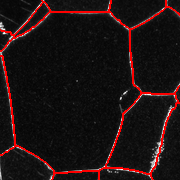
\includegraphics[width=0.30\linewidth]{fig/cca.pdf}}
\hspace{0.1em}
\subfloat[]{
\includegraphics[width=0.30\linewidth]{fig/ccf.pdf}}

\subfloat[]{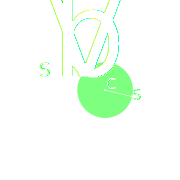
\includegraphics[width=0.30\linewidth]{fig/ccg.pdf}}
\hspace{0.1em}
\subfloat[]{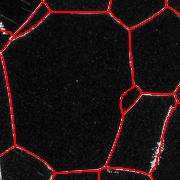
\includegraphics[width=0.30\linewidth]{fig/ccb.pdf}}
\caption{Automatic parameter selection.  \textbf{(a)}~A large segment
  containing an unsegmented structure near point~$c$.
  \textbf{(b-c)}~Selections of~$c$ at varying distances from the
  boundary of $S^V_b$, resulting in different estimations of~$s$.
  \textbf{(d)}~Result $S^{\tilde{V}}$ from selecting the~$c$ shown~(b)
  using the proposed parameter estimation method.} \label{fig:param}
\end{figure}

To obtain an estimation of $s$ we begin by setting $s$ a distance $0$
from the added point $c$.  We incrementally increase $s$ by a small
$\epsilon$ amount until the entire circle is within $\epsilon$
distance of the boundary of the containing segment $S^V_b$, as shown
by the arrow in \figsub{ex}{b-c}.  Empirically, the majority of
newly-appearing structures are near the boundary of a containing
structure $S^V_b$ (near a ``Y''-junction edge between structures),
this automatic approach well-handles such cases.  When the added point
$c$ falls directly on an edge, we default to requiring user-supplied
parameters in these less-common cases.  For simplicity, this approach
reduces to setting the distance $s$ to the nearest boundary pixel.
For estimating $d$, we scale it according to the value of $s$.
Specifically, we set $d = 2\cdot s$.  As shown in \sect{ex}, this
approach saves both time and effort.

%% Similar to this, we obtain
%% an estimation of $d$ by starting it at the estimated size of $s$, and
%% then incrementally increase it by $\epsilon$.  There is not a simple
%% stopping criterion to know undoubtedly that $d$ covers the entire
%% substructure desired.  However, we observe that if we separate the
%% containing segment into a background, and everything outside of the
%% containing segment into foreground, and we stop increasing $d$ when it
%% encompasses two, connected foreground regions, we tend to obtain a
%% large-enough value for $d$.  If this stopping condition never occurs,
%% we enforce a fixed maximum for $d$.  An illustration is given in
%% \fig{d-size}, where the $d$ size (blue circle) is not large enough in
%% \figsub{d-size}{a} and contains only a single connected foreground
%% component, whereas in \figsub{d-size}{b}, the $d$ size contains two
%% disjoint foreground regions, thus meeting the stopping criteria.
%% \begin{figure}[htbp]
%% \centering
%% \subfloat[Single foreground component]{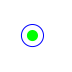
\includegraphics[width=0.30\linewidth]{fig/cce}}
%% \hspace{0.1em}
%% \subfloat[Two foreground components]{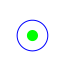
\includegraphics[width=0.30\linewidth]{fig/ccd.pdf}}
%% \caption{} \label{fig:d-size}
%% \end{figure}

\section{Experiments}
\label{sec:ex}

%% todo: add performance comparison

To evaluate the proposed interactive segmentation method, we use it to
segment a sequence of~$11$ microscopic titanium
images~\cite{rowenhorst:10} provided by Dave Rowenhorst, NRL.  We
measure the effort (\ie number of clicks) used to segment each slice
in the dataset, as well as the overall time expended by the user to
segment a slice.  The previous propagation approach~\cite{waggoner:11}
requires a complete segmentation as an initialization, so we include
the time required to segment this slice in the effort and time
required.  We present the proposed method both with and without using
the automatic parameter estimation discussed in \sect{param}.

For comparison, we use the readily-available ``intelligent scissors''
method~\cite{mortensen:95}.  Using this tool, we independently segment
all 11 slices from the same dataset, comparing effort (number of
clicks) and time.  In addition, we produce a hybrid of the proposed
method and the intelligent scissors method, which we call
``intelligent scissors + propagation'' in \fig{ex}.  This approach
uses the method from~\cite{waggoner:11} to propagate a segmentation
from an initial slice to the remaining slices, but it uses the
intelligent scissors tool~\cite{mortensen:95} to carry out the
interactive component instead of the interaction proposed in this
paper.

The results of this comparative experiment are shown in \fig{ex}.
Note that the first slice in propagated methods is used as an
initialization, so it requires significantly more effort and time to
segment compared with the remaining slices.
\begin{figure}[htbp]
\centering
\subfloat[Effort]{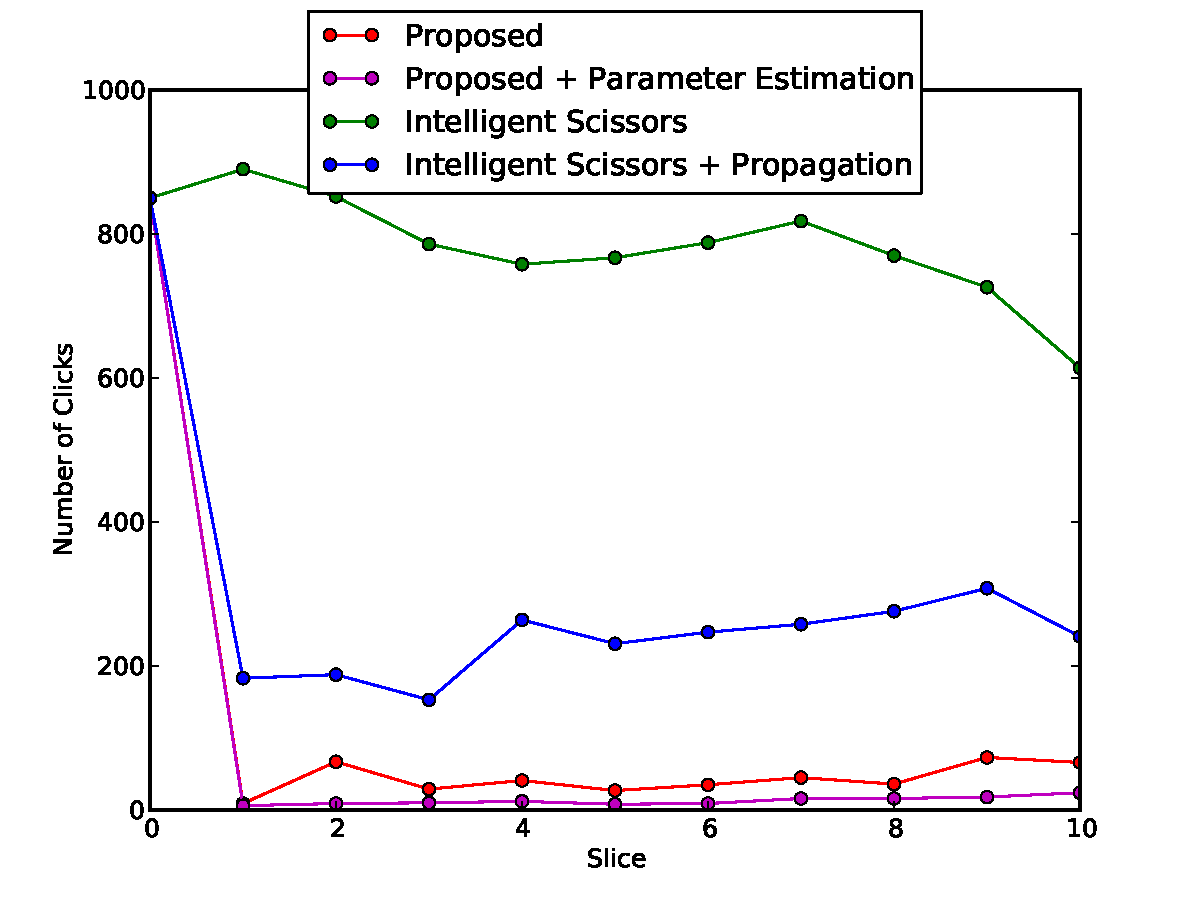
\includegraphics[width=0.48\linewidth]{fig/eval}}
\hspace{0.1em}
\subfloat[Time]{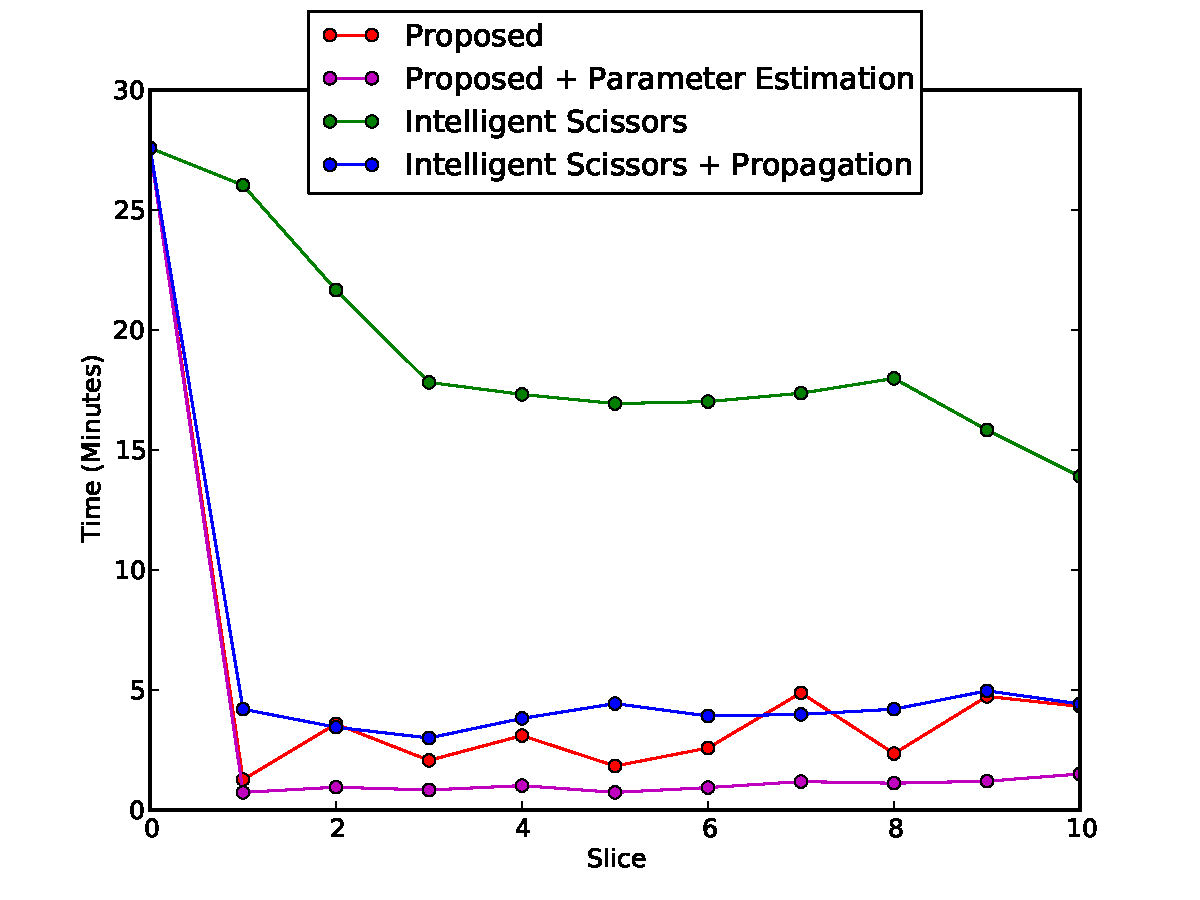
\includegraphics[width=0.48\linewidth]{fig/eval_time}}
\caption{Evaluation of \textbf{(a)} the amount of effort (number of
  clicks) and \textbf{(b)} time taken for a user to interactively
  segment the 11 sample slices.  Smaller values are better, for both
  figures.} \label{fig:ex}
\end{figure}
From \fig{ex}, the proposed method's propagation approach combined
with the interactivity discussed in this paper allows much more rapid
segmentation time ($< 5$ minutes in most cases) and with much less
effort ($< 100$ clicks in most cases) compared with the unpropagated
intelligent scissors method.  The intelligent scissors method, without
the benefit of an initialization, requires significantly more time and
effort.  The hybrid method fares better than the unpropagated method,
but it still requires greater effort than the proposed method.

Qualitative results for the proposed method are shown in \fig{qual}
where we show the erroneous segmentation, the human annotation, and
the updated segmentation.

\begin{figure}[htbp]
%% \renewcommand{\thesubfigure}{\thefigure.\arabic{subfigure}}
\setlength{\tabcolsep}{0.2em}

\centering

\subfloat[]{\begin{tabular}{ccc} 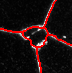
\includegraphics[width=0.15\linewidth]{fig/qual/a1} &
    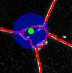
\includegraphics[width=0.15\linewidth]{fig/qual/a2} &
    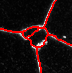
\includegraphics[width=0.15\linewidth]{fig/qual/a3} \end{tabular}} \hspace{1em}
\subfloat[]{\begin{tabular}{ccc} 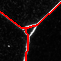
\includegraphics[width=0.15\linewidth]{fig/qual/b1} &
    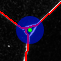
\includegraphics[width=0.15\linewidth]{fig/qual/b2} &
    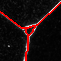
\includegraphics[width=0.15\linewidth]{fig/qual/b3} \end{tabular}}

\subfloat[]{\begin{tabular}{ccc} 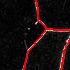
\includegraphics[width=0.15\linewidth]{fig/qual/c1} &
    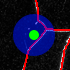
\includegraphics[width=0.15\linewidth]{fig/qual/c2} &
    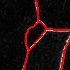
\includegraphics[width=0.15\linewidth]{fig/qual/c3} \end{tabular}} \hspace{1em}
\subfloat[]{\begin{tabular}{ccc} 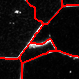
\includegraphics[width=0.15\linewidth]{fig/qual/d1} &
    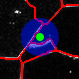
\includegraphics[width=0.15\linewidth]{fig/qual/d2} &
    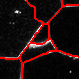
\includegraphics[width=0.15\linewidth]{fig/qual/d3} \end{tabular}}

\subfloat[]{\begin{tabular}{ccc} 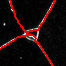
\includegraphics[width=0.15\linewidth]{fig/qual/e1} &
    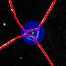
\includegraphics[width=0.15\linewidth]{fig/qual/e2} &
    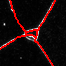
\includegraphics[width=0.15\linewidth]{fig/qual/e3} \end{tabular}} \hspace{1em}
\subfloat[]{\begin{tabular}{ccc} 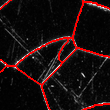
\includegraphics[width=0.15\linewidth]{fig/qual/f1} &
    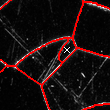
\includegraphics[width=0.15\linewidth]{fig/qual/f2} &
    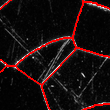
\includegraphics[width=0.15\linewidth]{fig/qual/f3} \end{tabular}}

\subfloat[]{\begin{tabular}{ccc} 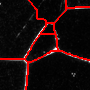
\includegraphics[width=0.15\linewidth]{fig/qual/g1} &
    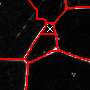
\includegraphics[width=0.15\linewidth]{fig/qual/g2} &
    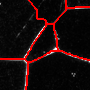
\includegraphics[width=0.15\linewidth]{fig/qual/g3} \end{tabular}} \hspace{1em}
\subfloat[]{\begin{tabular}{ccc} 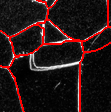
\includegraphics[width=0.15\linewidth]{fig/qual/h1} &
    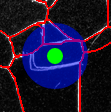
\includegraphics[width=0.15\linewidth]{fig/qual/h2} &
    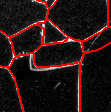
\includegraphics[width=0.15\linewidth]{fig/qual/h3} \end{tabular}}

\subfloat[]{\begin{tabular}{ccc} 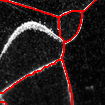
\includegraphics[width=0.15\linewidth]{fig/qual/i1} &
    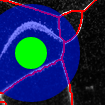
\includegraphics[width=0.15\linewidth]{fig/qual/i2} &
    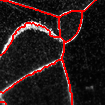
\includegraphics[width=0.15\linewidth]{fig/qual/i3} \end{tabular}} \hspace{1em}
\subfloat[]{\begin{tabular}{ccc} 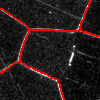
\includegraphics[width=0.15\linewidth]{fig/qual/j1} &
    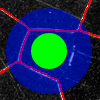
\includegraphics[width=0.15\linewidth]{fig/qual/j2} &
    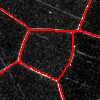
\includegraphics[width=0.15\linewidth]{fig/qual/j3} \end{tabular}}

\caption{Qualitative results showing original segmentation $S^V$
  (left), the human annotation (middle) with the seed pixels in green
  and dilation pixels in blue, and the updated $S^{\tilde{V}}$
  (right).  Note that (f) and (g) illustrate removal annotation with a
  small ``X'', and the remaining illustrate
  addition.} \label{fig:qual}
\end{figure}

\section{Conclusion}
\label{sec:conclusion}

We have presented an interactive segmentation method extended from a
propagated approach used in previous work.  By allowing the user to
interactively handle errors due to topology inconsistency when
propagating, we show that the time required to segment a materials
volume, as well as the overall effort (number of clicks) needed for
interaction, is much less than the comparison ``intelligent
scissors'' method used in popular image processing tools.  By
localizing the proposed interaction to local regions within the image,
we are able to obtain a fast, yet robust means to handle segmentation
errors within materials images that well-handles ambiguity within this
type of image.  Finally, by using a simple estimate for the small
number of parameters required by the interaction, we show that we can
further reduce the amount of time and effort needed by the proposed
approach.

\bibliography{matsci}
\bibliographystyle{spiebib}   %>>>> makes bibtex use spiebib.bst

\end{document} 
